\documentclass[11pt]{article}

\usepackage[margin=1in]{geometry}
\usepackage[utf8]{inputenc}
\usepackage[T1]{fontenc}
\usepackage{lmodern}
\usepackage{microtype}
\usepackage{booktabs}
\usepackage{longtable}
\usepackage{array}
\usepackage{enumitem}
\usepackage{amsmath}
\usepackage{xcolor}
\usepackage{hyperref}
\usepackage{titlesec}
\usepackage{graphicx}

\hypersetup{colorlinks=true, linkcolor=blue, urlcolor=blue}
\setlength{\parskip}{0.65em}
\setlength{\parindent}{0pt}
\titleformat{\section}{\large\bfseries\color{black}}{\thesection.}{0.5em}{}
\titleformat{\subsection}{\normalsize\bfseries\color{black}}{\thesubsection.}{0.5em}{}

\title{\textbf{AI Compute Accessibility Atlas:}\\
\large Analysis Approach, Stage 4 Causal Extension, Confounding Controls, and Causal Boundary}
\author{Project reference memo}
\date{March 13, 2026}

\begin{document}
\maketitle

\begin{center}
\fcolorbox{black}{gray!8}{\parbox{0.93\linewidth}{
\textbf{Purpose of this memo.} This note documents the \emph{Stage 4 causal-extension pass}. The goal was to see whether the current project could move from a strong spatial diagnosis toward a more credible causal claim. The answer is: \textbf{not yet}. The current snapshot lets us run meaningful stress tests against confounding, but it does not contain the ingredients for an event study or difference-in-differences design. Those stress tests are still useful, because they show how much of the original distance-to-AI association survives once we compare places more strictly.
}}
\end{center}

\section{What Stage 4 is trying to do}
Stage 1 established the descriptive geography. Stage 2 showed that the pattern is spatially structured and that the negative sign survives the project's original spatial-model setup. Stage 3 then interpreted that result carefully.

Stage 4 asks the next question:
\begin{quote}
Can the current dataset support a stronger causal interpretation, or does the association weaken once we compare like with like more aggressively?
\end{quote}

That is a different job from the earlier stages. It is not about making the pattern look clearer. It is about trying to break the pattern by adding stricter comparisons.

\section{What a real causal version would need}
A fully causal extension would normally use some kind of \emph{time variation}: cloud-region openings over time, before-and-after AI outcomes, and a comparison set of untreated cities. That would allow an event-study or diff-in-diff design.

The current repo does \textbf{not} contain those ingredients. What it contains is:
\begin{itemize}[leftmargin=*]
    \item current cloud-region locations,
    \item a current city-level OpenAlex overlay of recent AI works,
    \item city population and capital-status variables,
    \item and some country context from Natural Earth.
\end{itemize}

What it does \textbf{not} contain is:
\begin{itemize}[leftmargin=*]
    \item a city-year AI panel,
    \item time-stamped cloud-region openings,
    \item or a broader panel of pre-treatment confounders.
\end{itemize}

So the Stage 4 exercise in this memo is best understood as a \textbf{causal stress test}, not as a final identification design.

\section{What was actually done in the Stage 4 pass}
The extension proceeded in four steps.
\begin{enumerate}[leftmargin=*]
    \item Re-estimate the baseline relationship on the well-matched sample of 322 cities.
    \item Add richer geography and country controls to see whether the negative distance sign remains stable.
    \item Add \textbf{country fixed effects} and a direct within-country demeaned regression, which force the comparison to happen among cities inside the same country rather than across countries.
    \item Run simple treatment-style checks for being very close to compute (within 250 km or within 500 km), using doubly robust weighting as a loose matching-style robustness exercise.
\end{enumerate}

This is a good Stage 4 design for the current snapshot because it asks the right question: does the original association survive once the comparison gets harder?

\section{Sample used for the causal stress tests}
The main Stage 4 regressions use the 322 OpenAlex-city matches that fall within the report's 75 km match-quality threshold. The within-country diagnostic uses the 300 of those observations that belong to one of 41 countries with at least two matched cities. That matters because country fixed effects and country demeaning only make sense where there is more than one city to compare.

\section{The model battery}
\begin{longtable}{>{\raggedright\arraybackslash}p{0.24\linewidth} >{\raggedright\arraybackslash}p{0.54\linewidth} >{\raggedright\arraybackslash}p{0.14\linewidth}}
\toprule
\textbf{Model} & \textbf{What it asks} & \textbf{Distance coefficient} \\
\midrule
Stage4-B1 Baseline & Reproduces the core cross-sectional question with only log population added. & $-0.220$ \\
Stage4-B2 Country + subregion controls & Adds capital indicators, country GDP, country population, and subregion fixed effects. & $+0.124$ \\
Stage4-B3 Country fixed effects & Compares cities only within the same country, while still controlling for population and capital status. & $+0.151$ \\
Stage4-B4 Country FE + aggressive research-capacity control & Adds a strong city-level research proxy built from the top-institutions file. This is intentionally aggressive and may overcontrol. & $+0.179$ \\
Stage4-B5 Density-control stress test & Adds counts of nearby cloud regions and provider diversity within 500 km. & $+0.233$ \\
\bottomrule
\end{longtable}

All reported standard errors in this stage are clustered by country.

\section{The key result: the coefficient is not stable}
The single most important Stage 4 result is that the distance coefficient is \textbf{not stable} once the comparison is tightened.

In the baseline cross-sectional regression, the sign remains negative and lines up with the original report's direction: about $-0.220$ additional log-points in AI works for every extra 1{,}000 km from the nearest cloud region. But that estimate is already imprecise, with a 95\% interval of roughly $[-0.589, 0.149]$.

Once country and subregion structure are added, the coefficient flips positive to about $+0.124$. With country fixed effects, it becomes about $+0.151$. With an even more aggressive overcontrol for broader research capacity, it stays positive at about $+0.179$. None of these stricter estimates are statistically distinguishable from zero.

The practical meaning is simple:
\begin{quote}
\textbf{the original negative sign appears to be driven largely by between-country and between-region differences, not by a clean within-country gradient that would be easier to read causally.}
\end{quote}

\begin{figure}[htbp]
    \centering
    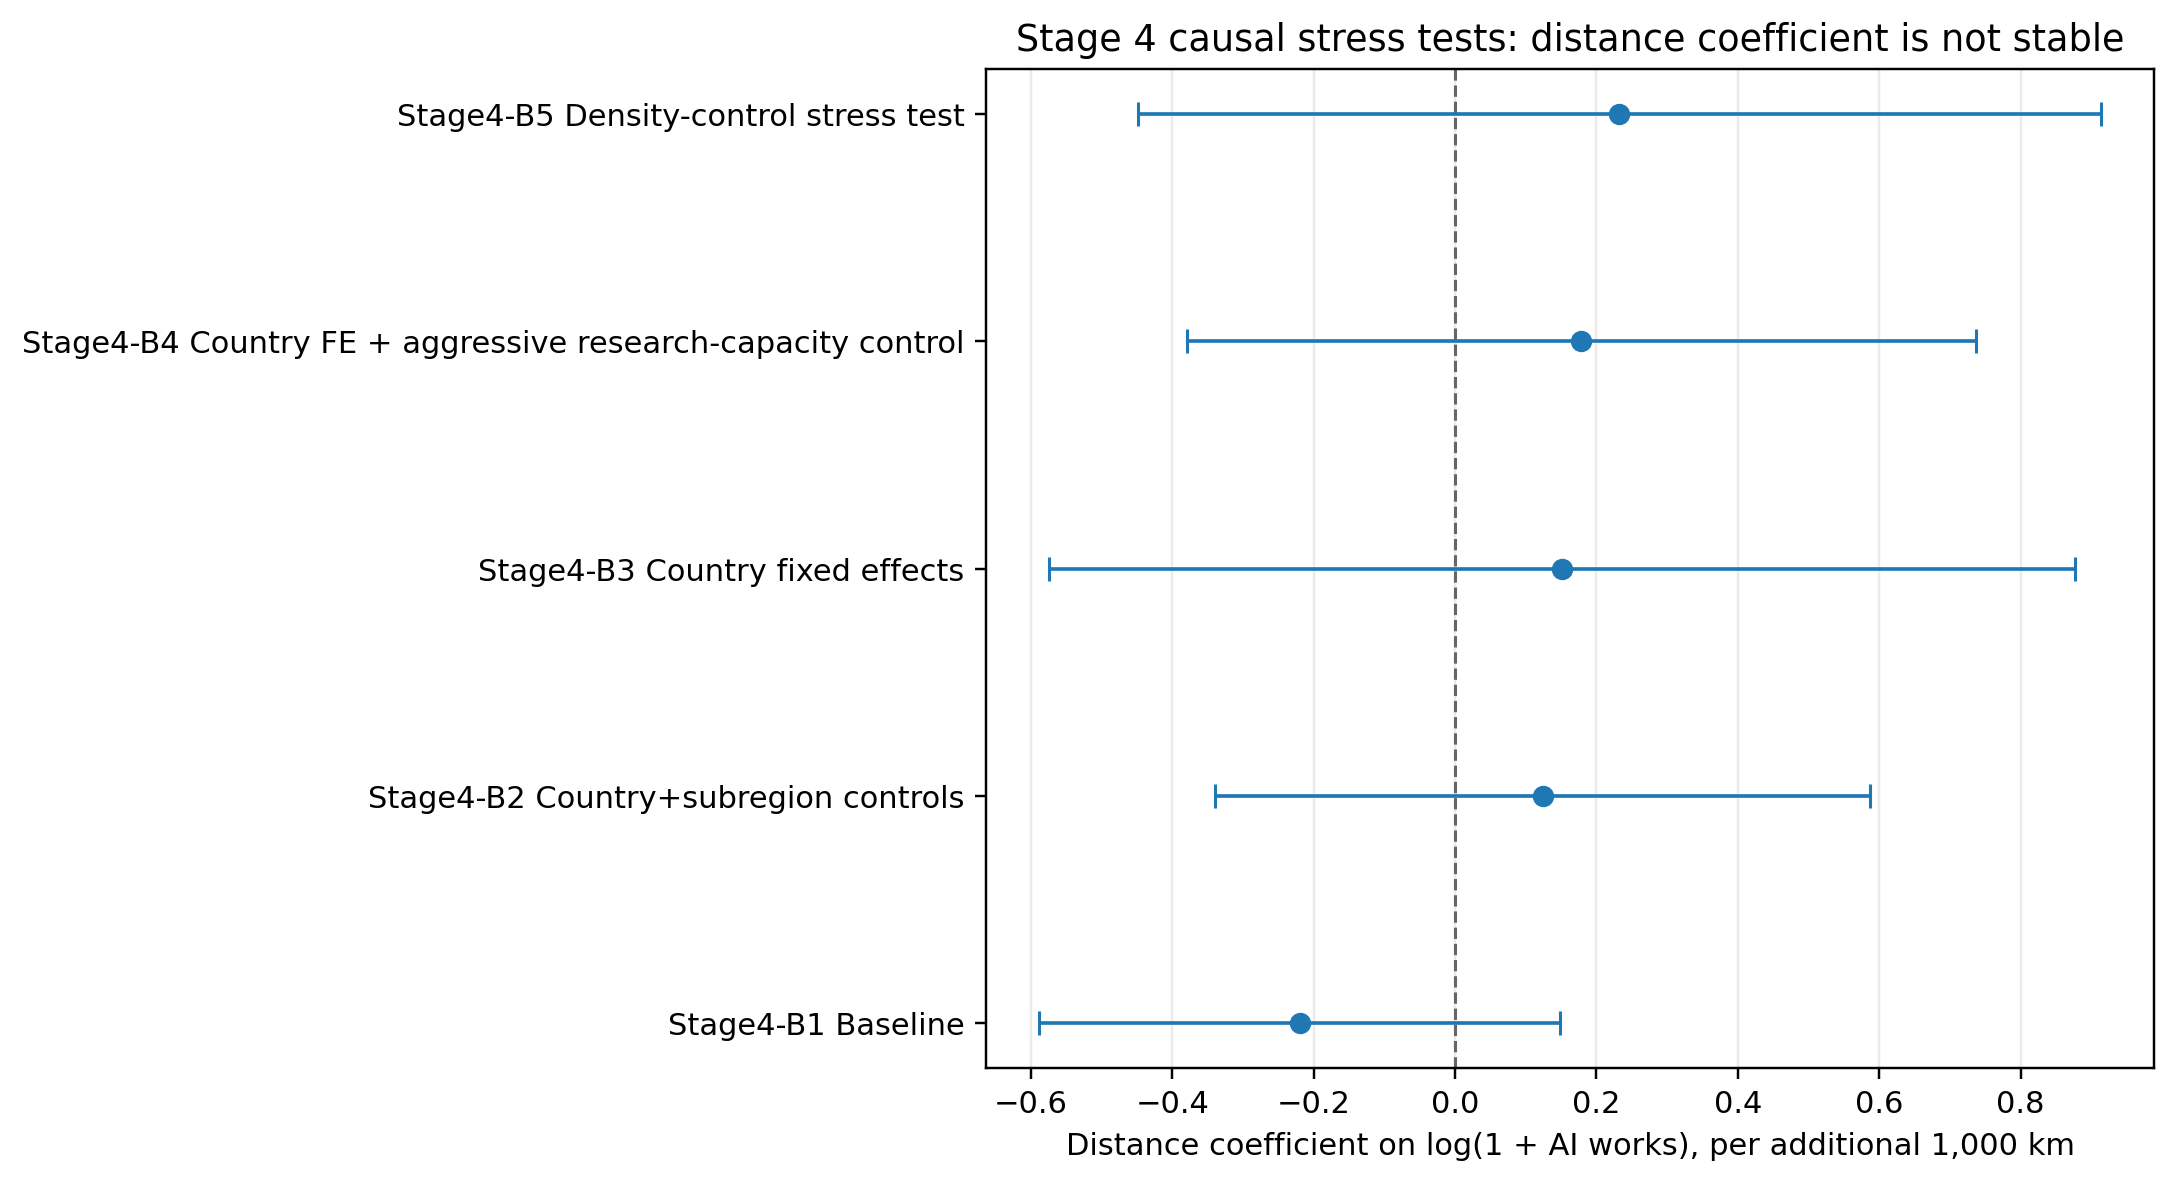
\includegraphics[width=0.95\linewidth]{../outputs/stage4/figures/fig_stage4_coef_stress_test.png}
    \caption{Stage 4 stress-test coefficients for distance to the nearest cloud region. The baseline model is negative, but richer controls and within-country comparisons pull the coefficient toward zero or positive values, with wide intervals crossing zero throughout.}
\end{figure}

\section{Within-country comparison}
A stronger causal-style question is not ``are far countries weaker in AI than near countries?'' but rather ``inside the same country, are the more compute-proximate cities systematically stronger in observed AI activity?''

The Stage 4 within-country demeaned regression addresses exactly that question. After removing country means, the estimated coefficient on distance is about $+0.088$ per additional 1{,}000 km, with $p \approx 0.787$. The simple demeaned correlation is about $-0.026$, which is very close to zero.

This does not prove that cloud distance is irrelevant. It does show that the current cross-sectional data do \textbf{not} provide a strong within-country signal that would support a causal reading.

\begin{figure}[htbp]
    \centering
    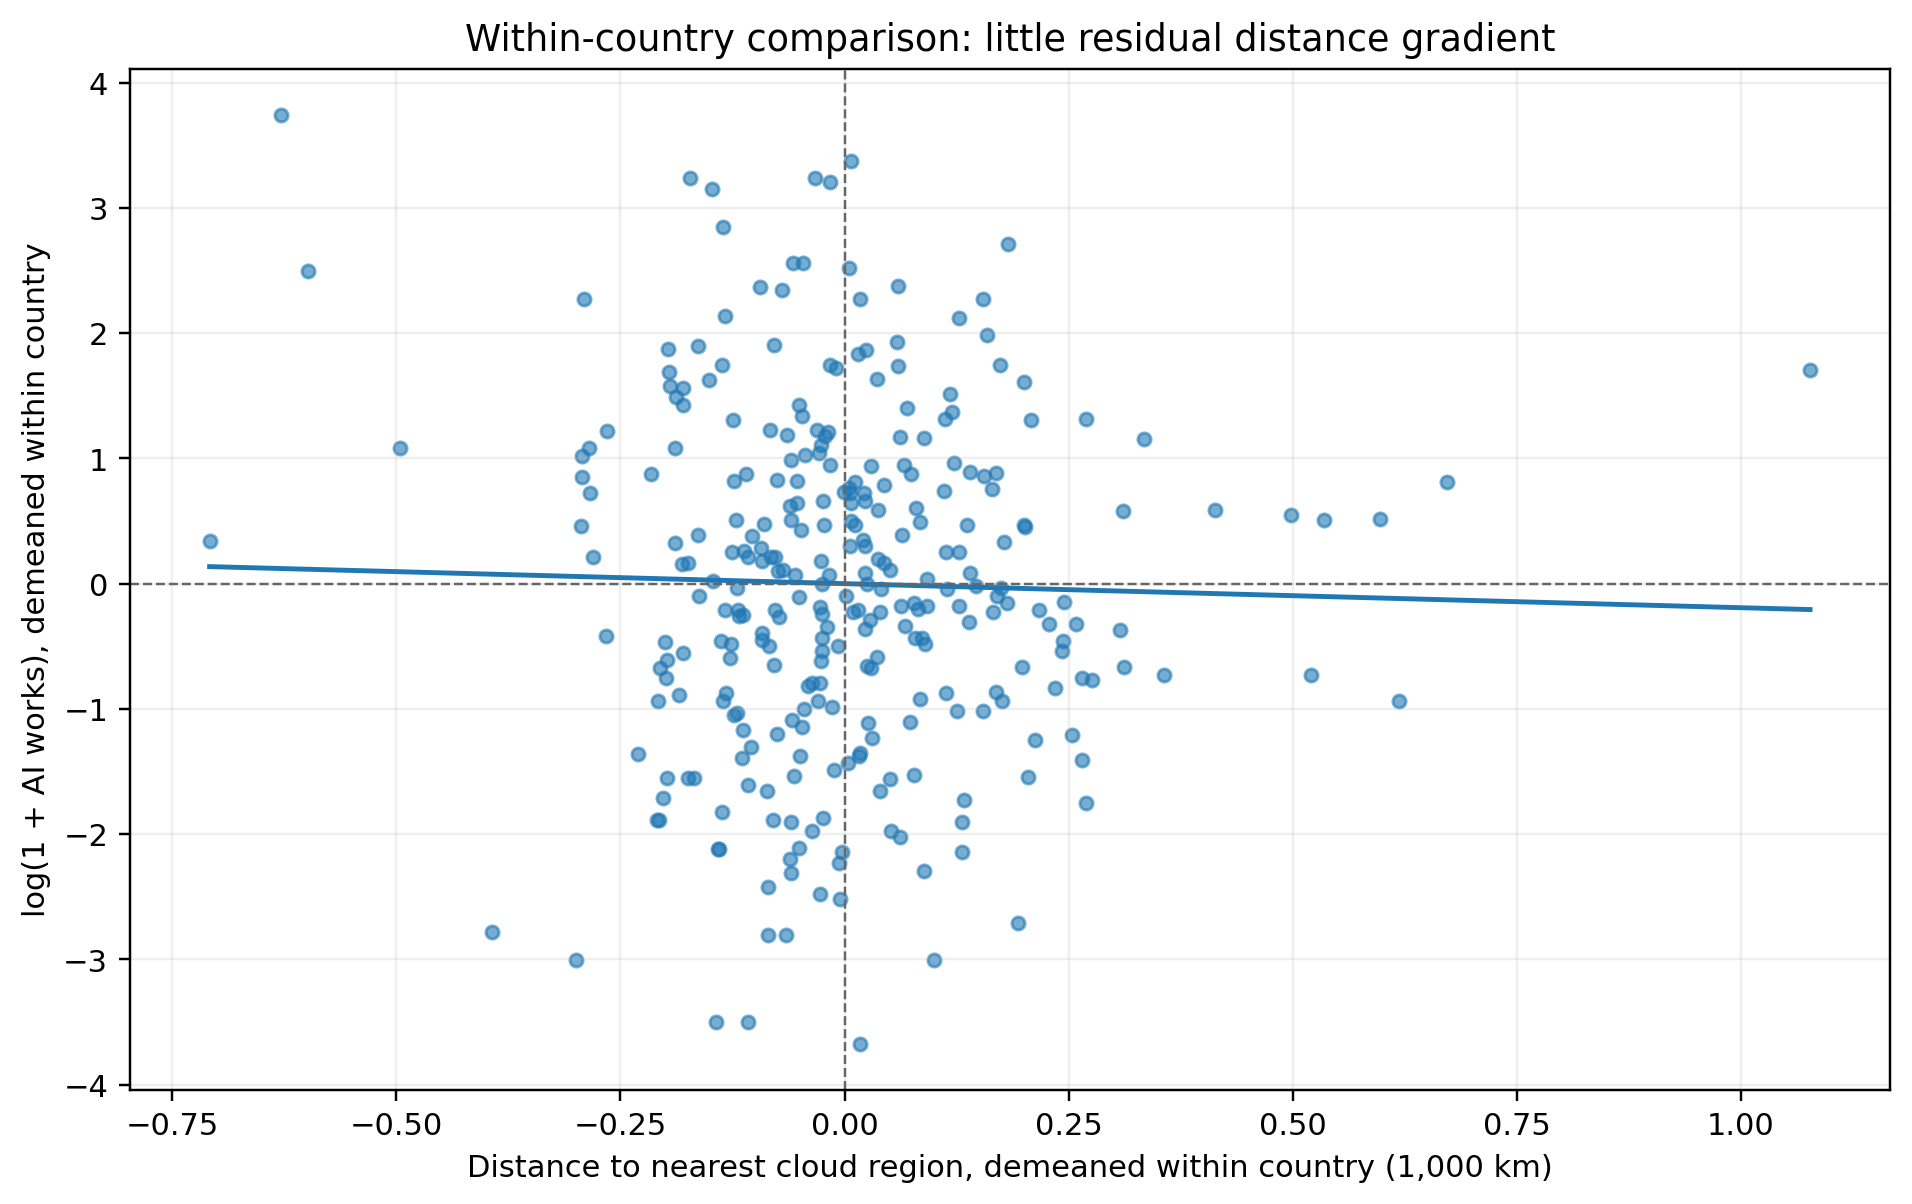
\includegraphics[width=0.92\linewidth]{../outputs/stage4/figures/fig_stage4_within_country_scatter.png}
    \caption{Within-country demeaned comparison. Once cities are compared relative to their own country's mean, the residual relationship between distance and AI works is weak and noisy.}
\end{figure}

\section{Treatment-style matching checks}
The project also tested a looser treatment framing: are cities very close to compute doing noticeably better than otherwise similar cities that are farther away?

Two thresholds were tested.
\begin{itemize}[leftmargin=*]
    \item \textbf{Within 250 km of a cloud region:} the naive treated-control difference is about $+0.070$ log-points ($p \approx 0.681$), while the doubly robust ATT estimate is about $-0.138$ ($p \approx 0.479$).
    \item \textbf{Within 500 km of a cloud region:} the naive difference is about $+0.088$ ($p \approx 0.609$), while the doubly robust ATT estimate is about $+0.170$ ($p \approx 0.411$).
\end{itemize}

The important thing here is not which sign one prefers. It is that the estimates are \textbf{unstable and imprecise}. That is exactly what one expects when the dataset is not rich enough to isolate a treatment effect cleanly.

\section{What these results do and do not mean}
\subsection{What Stage 4 does show}
Stage 4 shows three useful things.
\begin{enumerate}[leftmargin=*]
    \item The original negative association can be reproduced in a simple baseline model.
    \item That association is not robust to stricter geographic comparisons and country fixed effects.
    \item Therefore, the current data snapshot is not strong enough for a credible causal claim about compute proximity causing higher AI research activity.
\end{enumerate}

\subsection{What Stage 4 does not show}
Stage 4 does \textbf{not} show that compute accessibility is unimportant. It also does not show that the earlier stages were wrong. The earlier stages still support a meaningful descriptive and spatial-diagnostic conclusion.

What Stage 4 shows is narrower and more important for scientific discipline:
\begin{quote}
\textbf{the current evidence is better interpreted as an association that aligns with broad global geography than as a treatment effect that has survived serious causal scrutiny.}
\end{quote}

\section{Why the coefficient weakens}
There are at least three plausible reasons the coefficient weakens once the models become stricter.
\begin{enumerate}[leftmargin=*]
    \item \textbf{Between-country confounding.} Countries with stronger research systems, richer economies, larger technology sectors, or more cloud investment are also the ones more likely to host or sit near major regions.
    \item \textbf{Simplified treatment measurement.} Distance to the nearest region is a useful proxy, but it does not directly measure latency, service availability, pricing, regulation, data residency, or actual GPU access.
    \item \textbf{Outcome limitations.} The OpenAlex overlay measures one visible slice of AI activity, not the whole AI economy, and it is not a city-year panel.
\end{enumerate}

These are not minor caveats. They explain why a cross-sectional association can look meaningful descriptively but still fail to support causal language.

\section{Best supported conclusion after Stage 4}
After this extension, the strongest defensible conclusion is:
\begin{quote}
\textbf{The atlas still supports a meaningful spatial association between compute accessibility and observed AI activity at the global descriptive level, but the current data do not support a credible causal claim that greater proximity to cloud regions raises city-level AI research activity.}
\end{quote}

That is a stronger conclusion than simply saying ``causality is hard.'' It is based on an actual failed stress test: once stricter within-place comparisons are introduced, the negative distance signal no longer holds up.

\section{What a real next-step causal design would require}
A future Stage 4 that truly targets causality should add four ingredients.
\begin{enumerate}[leftmargin=*]
    \item \textbf{Cloud-region opening dates} for AWS, Azure, and GCP, ideally at the month or quarter level.
    \item \textbf{City-year AI outcomes,} whether from OpenAlex, patents, job postings, or another annual source.
    \item \textbf{Pre-treatment covariates over time,} such as population, national income, broadband or fiber proxies, electricity constraints, and broader research capacity.
    \item \textbf{A design built around shocks or timing,} such as event studies, diff-in-diff, or matched treated-control city panels.
\end{enumerate}

That is the path from a strong EIP atlas to a stronger causal paper.

\section{Bottom line}
Stage 4 was worth doing because it answered an important question honestly. It tried to promote the project from a compelling spatial diagnosis to a stronger causal claim, and it found that the data do not justify that promotion yet.

That is not a failure. It is a useful result. The project's central value remains intact: it reveals a hidden geography of compute accessibility and shows that this geography overlaps with where observed AI activity appears. But after the Stage 4 stress tests, the causal boundary is now sharper: the current atlas is best understood as a disciplined, policy-relevant spatial diagnosis, not as a proven estimate of what cloud-region proximity causes.

\end{document}
